% !TeX root = ../../thesis.tex
\chapter{Introduction}\label{ch:introduction}
\section{The quantum Hall effect}
In 1980, Klaus von Klitzing made a groundbreaking discovery in condensed matter physics by uncovering a remarkable phenomenon called the integer quantum Hall effect. He conducted experiments on a low-temperature silicon-based MOSFET under the influence of an external magnetic field. To his surprise, the Hall conductance induced by the magnetic field did not follow the classical linear dependence observed in the classical Hall effect, which is based on the Lorentz force acting on charged particles in a magnetic field. Instead, it formed distinct quantized plateaus (see figure \ref{fig:TopologicalOrderFigures}a).
\\\\
The materials exhibiting these Hall plateaus possessed intriguing new properties: they were classified by an integer, now known as the topological invariant or Chern number. Unlike conventional order parameters, this integer remained robust under local perturbations. Strikingly, this integer was typically not observable using local observables. It was only measurable by considering the total transversal conductivity of the entire system.
\\\\
Further investigations revealed that these quantized plateaus were manifestations of new phases of matter. They defied classification based on local order parameters, thereby challenging the conventional understanding of phases of matter described by Landau's paradigm.
\\\\
As the name suggests, the quantum Hall effect is inherently quantum mechanical in nature and is related to a topological property of the gapped many-body ground state. As such, the phenomenon is predominantly considered to be a zero-temperature phase of matter\footnote{Although certain caveats exist, such as the role of disorder, which allows the observation of quantum Hall plateaus even in situations without a gap.}. As these Hall plateaus were differentiated by some topological property of the many-body ground state, they were called topological phases of matter.
\\\\
For non-interacting electrons in periodic potentials, the topological property is characterized by the first Chern number of the Bloch bundle. However, for ground states of more general interacting Hamiltonians, distilling the properties that distinguish the phases is far more challenging and remains an active area of research. An example of such research is \cite{sopenko2023chiral} where the researchers produce examples of bosonic states that exhibit a similar kind of topological order.
\\\\
These integers are called topological properties, not just because they are Chern numbers of some bundle but because they are surprisingly robust. Any small and local perturbation of the gapped many-body Hamiltonian will leave the integers invariant just like a topological invariant remains unchanged under a continuous deformation of a topological space. For instance, it is impossible to continuously deform a 2-torus to a sphere because the 2-torus has a hole in it while the sphere does not. The amount of holes is a topological invariant that provides an obstruction to connecting topological spaces.
\begin{figure}
	\centering
	\begin{subfigure}[b]{0.45\textwidth}
		\centering
		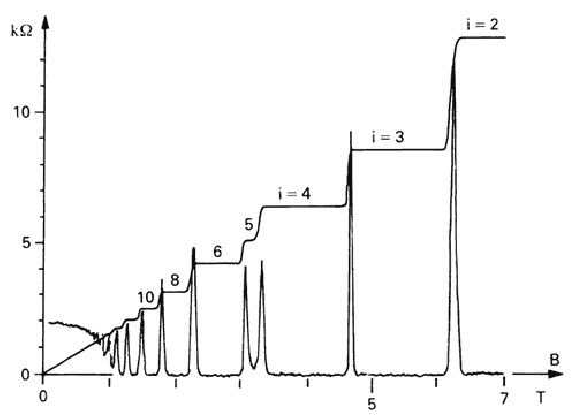
\includegraphics[width=\textwidth]{IntegerQHE.png}
		\caption{Integer quantum Hall effect (1980)}
	\end{subfigure}
	\hfill
	\begin{subfigure}[b]{0.45\textwidth}
		\centering
		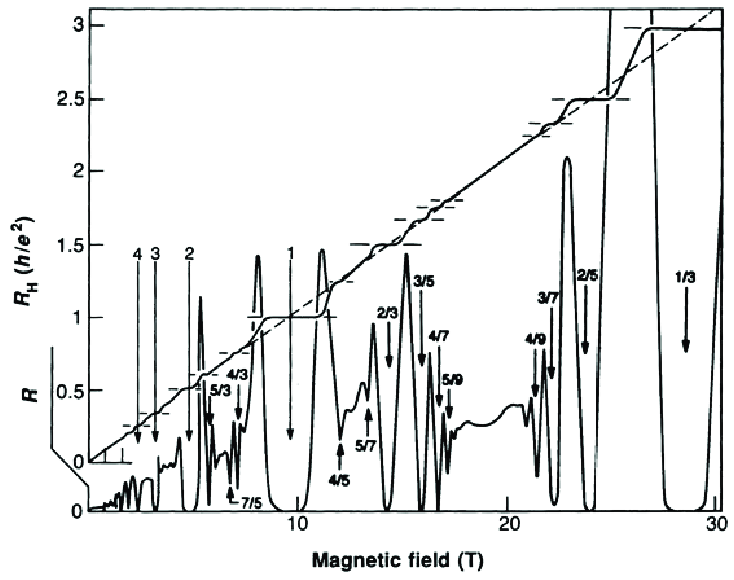
\includegraphics[width=\textwidth]{FractionalQHE.png}
		\caption{Fractional quantum Hall effect (1982)}
	\end{subfigure}
	\caption{Two examples of topological order, the integer quantum Hall effect displays invertible topological order while the fractional quantum Hall effect displays both invertible and anyonic topological order.}
	\label{fig:TopologicalOrderFigures}
\end{figure}
\section{Topological phases of matter}
Later on, many more such phases of matter were found. They were all characterized by topological invariants. The most famous examples are the fractional quantum Hall effect (see figure \ref{fig:TopologicalOrderFigures}b), measured in 1982, and the theoretical toric code\cite{Kitaev_2003} model.
\\\\
These phases of matter exhibit what we now call anyonic topological order. They get their name from the fact that the excitations of a state with anyonic topological order have anyonic braiding statistics. One of their striking properties is that the ground state degeneracy of a macroscopically large sample depends on the topology of the surface one puts it on. If one has a two-dimensional material exhibiting anyonic topological order, then wrapping the material on the 2-torus will give a different ground state degeneracy than if one were to wrap it on a sphere. In general, this ground state degeneracy depends on the homology of the surface.
\\\\
More recently a more sophisticated method was developed to distinguish the different anyonic phases of matter (mathematically) using braided tensor categories constructed out of so-called superselection sectors. These braided tensor categories are again a topological invariant of a ground state. Similarly to what occurred in the integer quantum Hall phase, no smooth deformation of the gapped many-body Hamiltonian that leaves the gap open can change this category.
\\\\
In the following years, many theoretical attempts were made at classifying all possible topological phases of matter (just as the Landau theory classifies symmetry-breaking phases). We now have a theory of invertible topological order, which is believed to be related to the integer quantum Hall effect, and anyonic topological order, associated with the fractional quantum Hall effect.
\section{Classification of topological order through gapped phases of matter}
The robustness of the above-mentioned topological orders already gives a hint at how one should approach the classification problem of topological phases of matter. Consider the lattice $\ZZ^d$ (where $d$ is the spatial dimension) and take all gapped Hamiltonians that are a sum (where the sum is over the lattice) of local terms. Two states are in the same phase if one is able to smoothly deform the terms of their parent Hamiltonians into one another without closing the gap. This gives an equivalence class on all gapped Hamiltonians that divides the space of Hamiltonians with a unique gapped ground state in different classes (a quick sketch of these classes is given in figure \ref{fig:SymmetryEnrichedIntroduction}a).
\\\\
The topological properties of the ground states that we mentioned before (like the Chern number or the braided tensor categories) are then obstructions to connecting two parent Hamiltonians. If one has two Hamiltonians whose gapped ground states have different topological properties it becomes impossible to connect them. In other words, two states with different transversal Hall conductance or different braided tensor categories have to be in different gapped phases of matter.
\begin{figure}
	\begin{subfigure}[b]{0.45\textwidth}
		\centering
		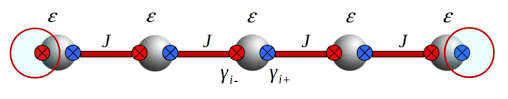
\includegraphics[width=\textwidth]{MajoranaEdgeModes.png}
		\caption{Majorana edge modes (first reported to be found in 2012 but data was not conclusive). For more information on the fermionic SPT classification see \cite{Bourne_2021}.}
	\end{subfigure}
	\hfil
	\begin{subfigure}[b]{0.45\textwidth}
		\centering
		\includegraphics[width=\textwidth]{Fermi-Hubbard Ladders.pdf}
		\caption{Fermi Hubbard ladders (see \cite{sompet2022realizing}). This is an example of the Haldane phase that we will discuss in Section \ref{sec:an-example-in-1d-the-haldane-phase}. This is from an experiment done in 2021.}
	\end{subfigure}
	\caption{Two examples of symmetry-protected topological order.}
	\label{fig:SymmetryProtectedTopologicalOrderFigures}
\end{figure}
\section{Symmetry protected topological order}
\begin{figure}
	\begin{subfigure}[b]{0.45\textwidth}
		\centering
		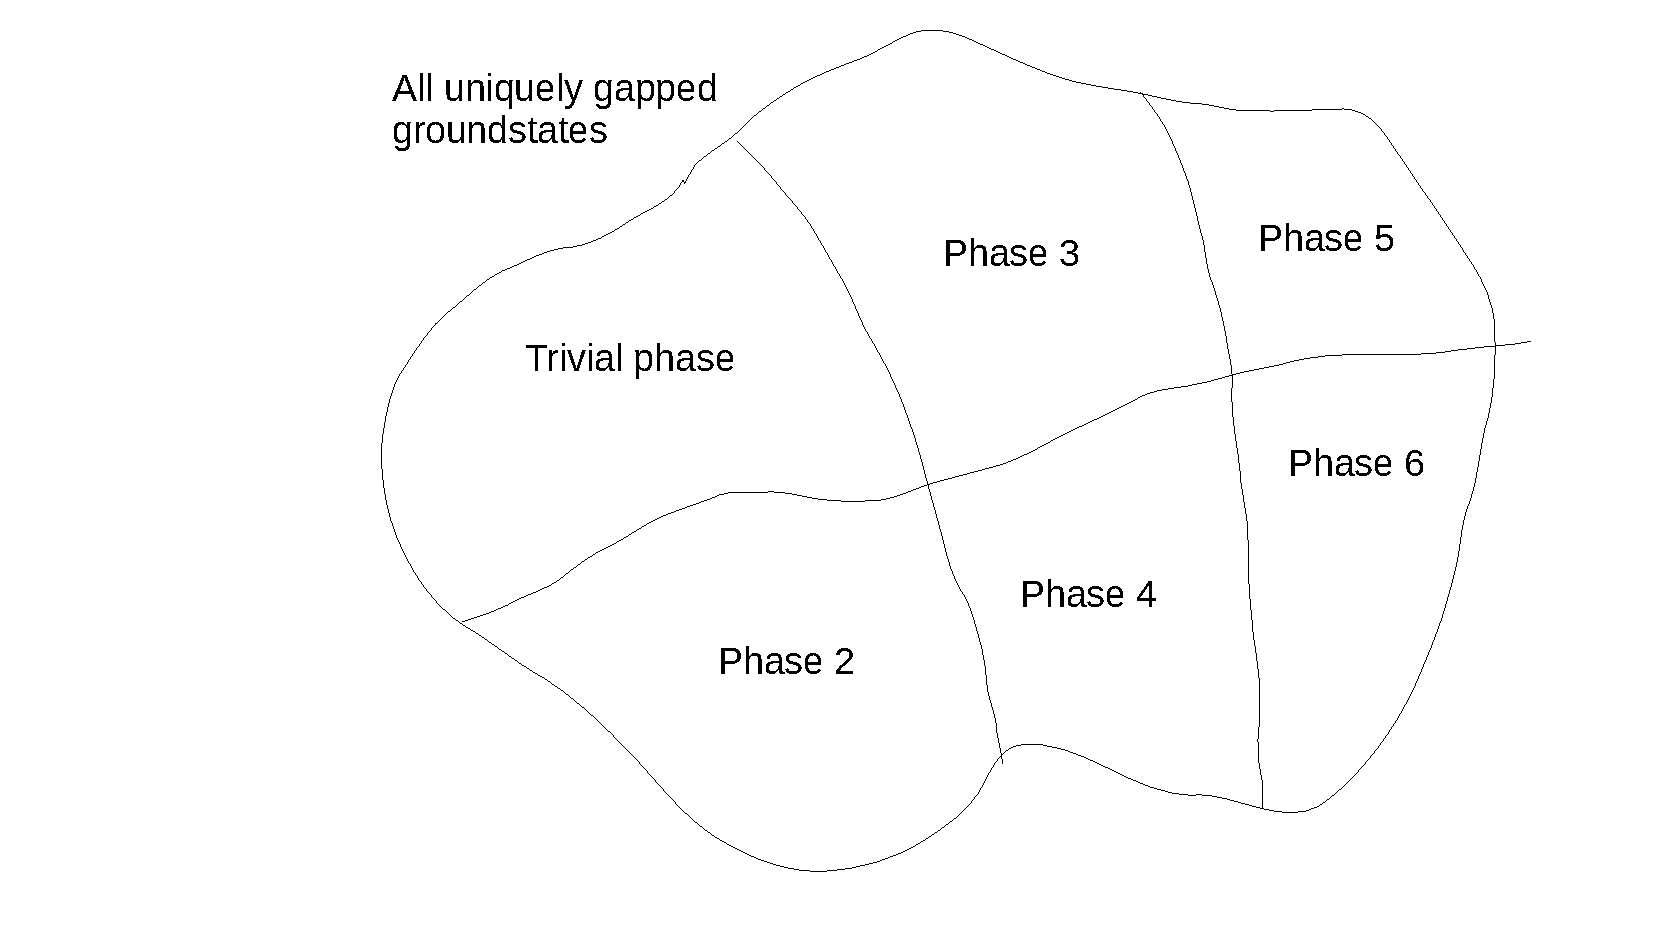
\includegraphics[width=\textwidth]{GappedPhasesOfQuantumMatter.pdf}
		\caption{Without a symmetry.}
	\end{subfigure}
	\hfil
	\begin{subfigure}[b]{0.45\textwidth}
		\centering
		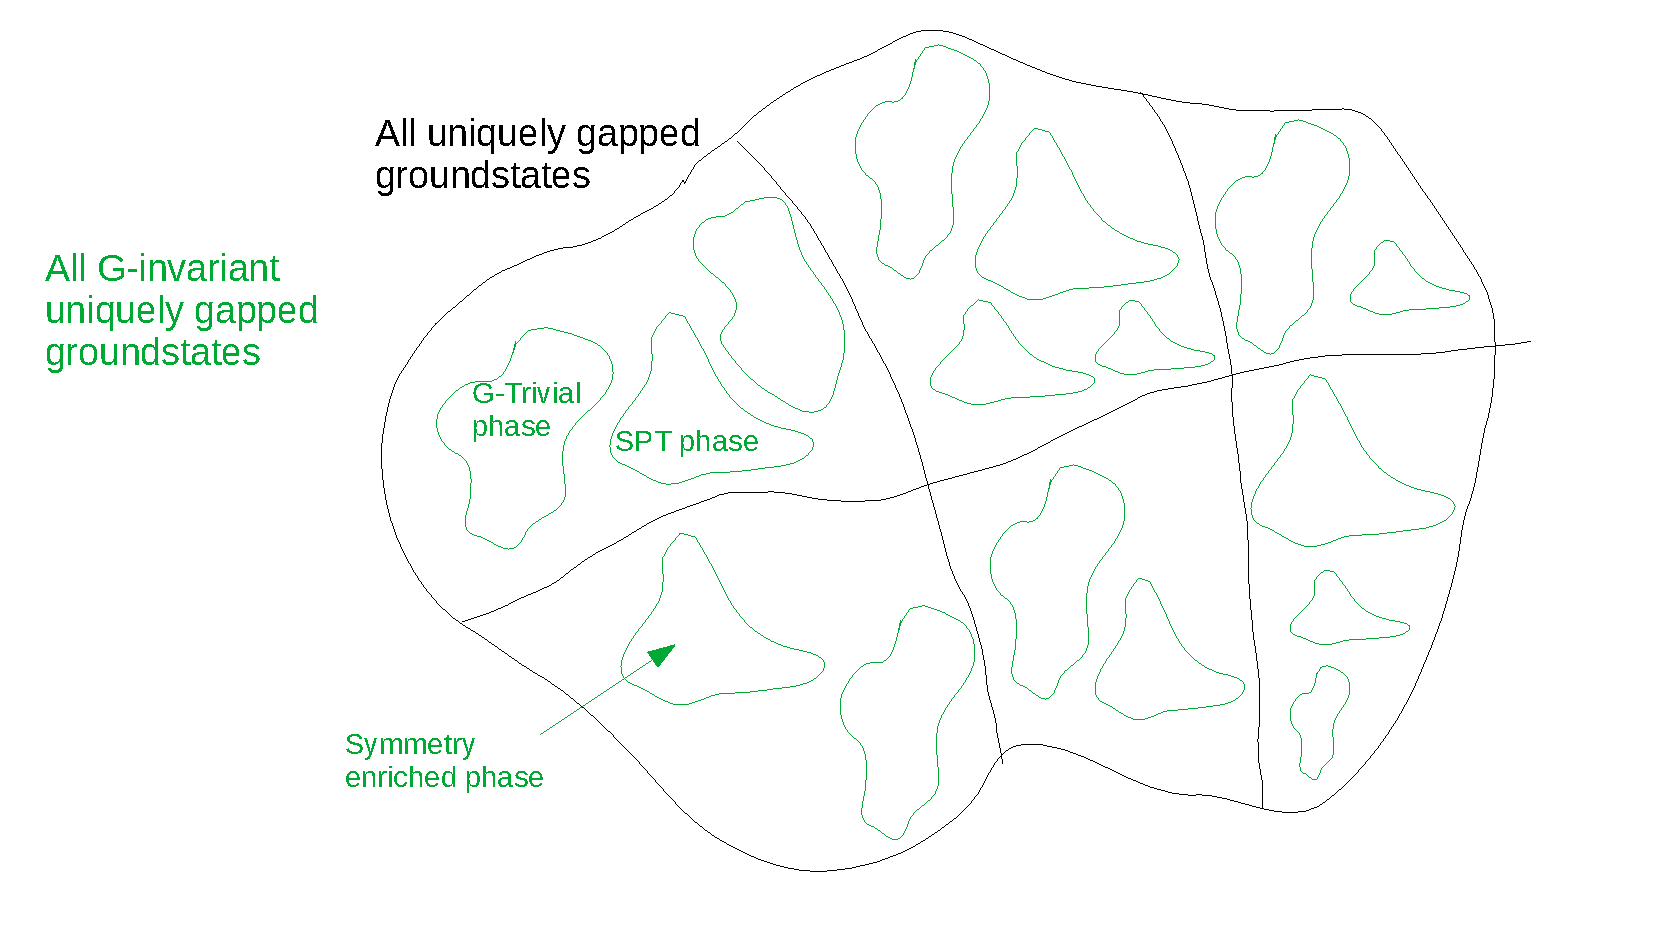
\includegraphics[width=\textwidth]{Symmetry_Enriched_Phases.pdf}
		\caption{With a symmetry.}
	\end{subfigure}
	\caption{This figure depicts the division of gapped Hamiltonians into gapped phases of matter. The first picture is without a symmetry and different phases can belong to different topological indices (e.g. a state with a nontrivial quantum Hall conductance has to be in a different phase). The second picture shows how this changes when we add a symmetry. A G-invariant part of the trivial phase is then called an SPT phase while the G-invariant part of another phase is called a symmetry-enriched phase.}
	\label{fig:SymmetryEnrichedIntroduction}
\end{figure}
This rich class of gapped phases of matter is certainly interesting by itself and has sparked a wide interest in both the theoretical and experimental communities. The work here is far from being completed. However, to go to the topics presented in the rest of this thesis we will need one additional element, a symmetry.
\\\\
Some topological properties of gapped ground states are only well-defined if one defines a symmetry. In an isolated and confined system where particles are not able to escape, there is a preserved electric charge for instance. This implies that it is impossible to smoothly deform a system without charge to one with charge while preserving the symmetry (in fact this is the simplest form of symmetry-protected topological order and is discussed in Section \ref{sec:zero-dimensional-spts}).
\\\\
The addition of a symmetry changes the landscape of gapped phases of matter completely. Imposing a symmetry means that one only looks at the gapped Hamiltonians that contain exclusively $G$-invariant local terms. Additionally, one changes the equivalence class to only include smooth deformations of the local terms that are $G$-invariant. In this case, the classes fall apart in smaller subclasses.
\\\\
The subclasses that are obtained this way are called the classes of symmetry-enriched topological order (see figure \ref{fig:SymmetryEnrichedIntroduction}b for a graphical depiction of such phases). It should be noted that the classes do not cross boundaries, two $G$-invariant Hamiltonians that are in different quantum phases of matter cannot be in the same symmetry-enriched class. This means that our topological indices factorize, there is a topological index related to the ordinary topological order and an additional index related to the symmetry. \footnote{However, the space in which the symmetry enrichment indices are situated can differ for each topological phase. This is depicted in figure \ref{fig:SymmetryEnrichedIntroduction}b by not having the same amount of green parts for each black part.}
\\\\
In this manuscript, we will mainly focus on the symmetry enrichment of the trivial quantum phase of matter (see figure \ref{fig:ConnectedComponents}). The equivalence classes obtained here are then called the symmetry-protected topological (or SPT) phases because they are only protected because of the symmetry and are trivial without it. Some well-known examples of symmetry-protected topological order are the Majorana edge mode model (see figure \ref{fig:SymmetryProtectedTopologicalOrderFigures}a), protected by fermion statistics, and the Haldane phase (see figure \ref{fig:SymmetryProtectedTopologicalOrderFigures}b), protected by the rotational symmetry $SO(3)$. While the Majorana edge mode model remains mainly theoretical, the Haldane phase has been experimentally\cite{sompet2022realizing} observed.

\section{What is in this thesis}
The work in this thesis aims at improving our understanding of bosonic symmetry-protected topological order in various specific cases.
\paragraph{Chapter \ref{sec:SPT_Order_In_A_Nutshell}:}This chapter provides a concrete and simple framework for looking at the trivial gapped phase of matter by considering finite depth quantum circuits. It then uses this to introduce the notions of short-ranged entangled (SRE) states. Afterwards, we define the on-site group action and use this to define symmetry-protected topological (SPT) states. It then proceeds with some examples. First, we discuss zero-dimensional SPT order (which just amounts to a preservation of charge), then we explain an example of SPT order in 1d called the Haldane phase. We then talk about the definition of group cohomology groups in which all our SPT indices take values. Finally, we will show how these finite depth quantum circuits can be used to define the notion of loops and the notion of homotopy of loops. We show that to such a loop, we can associate a boundary state.
\paragraph{Chapter \ref{ch:Tools_For_Quantum_many_Body}:}This chapter provides the necessary mathematical background to understand the rest of the paper. We first define various objects and concepts. We then use this new formalism to properly define the $H^2(G,\TT)$-valued index associated to SPT states over $\ZZ$.
\paragraph{Chapter \ref{ch:LoopSPT}:}This chapter is based on the paper \hyperref[mySecondPaper]{[b]}. It features a generalization of the loop SPT index constructed in Section \ref{sec:loops-of-spts} called the charge pumping index. It is a generalization of the known $\ZZ$-valued index for the Thouless pump. It then proves the existence and completeness of this index.
\paragraph{Chapter \ref{ch:TranslationSPT}:}This chapter is based on the paper \hyperref[myFirstPaper]{[a]}. It considers SPT states in two spatial dimensions and looks at how the SPT classification changes if one imposes additional translation symmetries. It proves that these indices are well-defined.

%%%%%%%%%%%%%%%%%%%%%%%%%%%%%%%%%%%%%%%%%%%%%%%%%%
% Keep the following \cleardoublepage at the end of this file, 
% otherwise \includeonly includes empty pages.
\cleardoublepage

% vim: tw=70 nocindent expandtab foldmethod=marker foldmarker={{{}{,}{}}}